\documentclass[11pt,a4paper]{article}

% --- Codificación, idioma y tipografía ---
\usepackage[utf8]{inputenc}
\usepackage[T1]{fontenc}
\usepackage[spanish,es-nodecimaldot]{babel}
\usepackage{lmodern}
\usepackage[scaled=0.92]{helvet}
\usepackage{microtype}

% --- Geometría amplia y limpia ---
\usepackage[
  a4paper,
  top=2.6cm,
  bottom=2.6cm,
  left=2.5cm,
  right=2.5cm,
  headheight=20pt,
  headsep=16pt,
  footskip=26pt
]{geometry}

\usepackage{setspace}
\setstretch{1.18}
\setlength{\parskip}{0.55em}
\setlength{\parindent}{0pt}

% --- Paquetes gráficos y de tablas (con [table] en xcolor para \rowcolor) ---
\usepackage[table]{xcolor}
\usepackage{graphicx}
\usepackage{subcaption}
\usepackage{booktabs}
\usepackage{tabularx}
\usepackage{array}
\usepackage{amsmath,amssymb}
\usepackage{enumitem}
\usepackage{float}
\usepackage{fancyhdr}
\usepackage{lastpage}
\usepackage{titlesec}
\usepackage[most]{tcolorbox}
\usepackage{hyperref}
\usepackage{url}
\usepackage{caption}
\usepackage{tikz}
\usetikzlibrary{arrows.meta, positioning}

% =============================================================================
% CONFIGURACIÓN DE ENLACES OFICIALES (Coloca aquí el link de tu video)
% =============================================================================
\newcommand{\dashboardlink}{\url{https://galektato.github.io/Agrotec-Amanteca/}}
\newcommand{\repolink}{\url{https://github.com/GalekTato/Agrotec-Amanteca}}
\newcommand{\videolink}{\url{https://youtu.be/ENLACE_VIDEO_DEMOSTRATIVO}} % <-- Pon aquí tu enlace de YouTube/Drive

% --- Paleta de color Editorial Agro-Tech ---
\definecolor{forestdeep}{HTML}{0B3B2D}   % Verde bosque profundo
\definecolor{emeraldmid}{HTML}{107C5C}   % Esmeralda vivo
\definecolor{mintsoft}{HTML}{EBF5F0}     % Fondo menta suave
\definecolor{amberwarm}{HTML}{D97706}    % Ámbar / Cebada dorada
\definecolor{amberlight}{HTML}{FEF3C7}   % Fondo ámbar suave
\definecolor{slatedark}{HTML}{1E293B}    % Gris pizarra oscuro
\definecolor{slatemuted}{HTML}{64748B}   % Gris medio
\definecolor{surfacebg}{HTML}{F8FAFC}    % Gris perla de fondo
\definecolor{borderline}{HTML}{CBD5E1}   % Bordes sutiles

\color{slatedark}

\hypersetup{
  colorlinks=true,
  linkcolor=emeraldmid,
  urlcolor=amberwarm,
  citecolor=forestdeep,
  pdftitle={Agrotec-Amanteca | Reporte Técnico Reto AgroCebada FIRA 2026},
  pdfauthor={Equipo Agrotec-Amanteca}
}

% --- Encabezados y pies de página (Numeración infalible con LastPage) ---
\pagestyle{fancy}
\fancyhf{}
\renewcommand{\headrulewidth}{0pt}
\lhead{%
  \begin{tikzpicture}[baseline=(current bounding box.base)]
    \fill[amberwarm] (0,0) rectangle (0.16,0.26);
    \node[anchor=west, font=\sffamily\footnotesize\bfseries, text=forestdeep] at (0.26,0.13) {AGROTEC-AMANTECA};
    \node[anchor=west, font=\sffamily\footnotesize, text=slatemuted] at (3.60,0.13) {| \ Reto AgroCebada FIRA 2026};
  \end{tikzpicture}%
}
\rhead{\sffamily\footnotesize\color{emeraldmid}\textbf{\nouppercase{\leftmark}}}
\lfoot{\sffamily\scriptsize\color{slatemuted}Predicción Geoespacial del Rendimiento de Cebada}
\rfoot{\sffamily\footnotesize\color{slatemuted}Página \textcolor{forestdeep}{\textbf{\thepage}} de \textcolor{forestdeep}{\textbf{\pageref*{LastPage}}}}

% --- Formato de Títulos ---
\titleformat{\section}
  {\sffamily\Large\bfseries\color{forestdeep}}
  {\tcbox[colback=forestdeep, colframe=forestdeep, coltext=white, on line, boxsep=2pt, left=5pt, right=5pt, top=2pt, bottom=2pt, arc=2pt]{\sffamily\normalsize\thesection}}
  {0.6em}
  {}
  [\vspace{0.2em}{\color{amberwarm}\titlerule[1.2pt]}\vspace{0.1em}]

\titleformat{\subsection}
  {\sffamily\large\bfseries\color{emeraldmid}}
  {\textcolor{amberwarm}{\rule[0.1em]{0.35em}{0.65em}}\hspace{0.4em}\thesubsection}
  {0.4em}
  {}

\titlespacing*{\section}{0pt}{2.8ex plus 0.6ex minus 0.2ex}{1.3ex}
\titlespacing*{\subsection}{0pt}{2.0ex plus 0.4ex minus 0.2ex}{0.7ex}

% --- Listas y leyendas ---
\setlist[itemize]{leftmargin=1.5em, itemsep=3pt, topsep=3pt, label=\textcolor{amberwarm}{$\blacktriangleright$}}
\setlist[enumerate]{leftmargin=1.8em, itemsep=3pt, topsep=3pt, font=\sffamily\bfseries\color{forestdeep}}
\captionsetup{font={small,sf}, labelfont={bf,color=forestdeep}, textfont={color=slatemuted}, skip=6pt}

% --- Comandos auxiliares ---
\newcommand{\code}[1]{\tcbox[on line, boxsep=1pt, left=3pt, right=3pt, top=1pt, bottom=1pt, colback=mintsoft, colframe=mintsoft, arc=2pt]{\texttt{\footnotesize\color{forestdeep}#1}}}

\newcommand{\weightbar}[3]{%
  \noindent{\sffamily\footnotesize\textbf{#1} \hfill \textcolor{forestdeep}{\textbf{#2\%}}}\\[-0.55em]
  \begin{tikzpicture}
    \fill[surfacebg, rounded corners=1.5pt] (0,0) rectangle (\linewidth, 0.20);
    \fill[#3, rounded corners=1.5pt] (0,0) rectangle (#2*0.01\linewidth, 0.20);
  \end{tikzpicture}\vspace{0.15em}%
}

\begin{document}

% =============================================================================
% PORTADA EDITORIAL EN 1 SOLA PÁGINA (SIN DESBORDAMIENTOS NI AFICHES)
% =============================================================================
\begin{titlepage}
\thispagestyle{empty}

% Barra superior de identidad
\noindent
\begin{tikzpicture}
  \fill[forestdeep] (0,0) rectangle (0.72\textwidth, 0.35cm);
  \fill[amberwarm] (0.72\textwidth,0) rectangle (\textwidth, 0.35cm);
\end{tikzpicture}

\vspace{0.8cm}

% Encabezado: Logo + Convocatoria
\noindent
\begin{minipage}[c]{0.18\textwidth}
  \IfFileExists{frontend/public/logo_agrotec_amanteca.jpg}
    {
\includegraphics[width=2.5cm]{frontend/public/logo_agrotec_amanteca.jpg}}
    {\begin{tcolorbox}[width=2.4cm, height=2.4cm, colback=forestdeep, colframe=amberwarm, boxrule=1.5pt, arc=6pt, valign=center, halign=center]
       \sffamily\bfseries\footnotesize\color{white}AGROTEC\\[-2pt]\color{amberwarm}AMANTECA
     \end{tcolorbox}}
\end{minipage}%
\begin{minipage}[c]{0.82\textwidth}
  {\sffamily\small\bfseries\color{amberwarm} CONVOCATORIA NACIONAL $\cdot$ RETO AGROCEBADA FIRA 2026}\\[3pt]
  {\sffamily\Large\bfseries\color{forestdeep} Equipo Agrotec-Amanteca}\\[2pt]
  {\sffamily\footnotesize\color{slatemuted} Reporte Técnico Oficial de Modelado Predictivo e Interfaz Tecnológica}
\end{minipage}

\vspace{1.6cm}

% Bloque central del Título con barra lateral izquierda limpia
\begin{tcolorbox}[
  enhanced,
  colback=white,
  colframe=white,
  borderline west={4.5pt}{0pt}{forestdeep},
  left=16pt, right=4pt, top=6pt, bottom=6pt,
  boxrule=0pt, sharp corners
]
  {\sffamily\fontsize{24}{30}\selectfont\bfseries\color{forestdeep}
  Sistema Geoespacial e Inteligencia Artificial para la Predicción del Rendimiento de Cebada\par}

  \vspace{0.45cm}
  {\color{amberwarm}\rule{4.0cm}{2.2pt}}
  \vspace{0.45cm}

  {\sffamily\large\color{slatemuted}
  Arquitectura de ensamble libre de fuga de datos (\textit{Leak-Free Smart-Pearson + IDW}), proyectada en coordenadas métricas UTM Zona 14N con calibración empírica de incertidumbre y simulador agroclimático interactivo.\par}
\end{tcolorbox}

\vspace{1.0cm}

% Resumen Ejecutivo Breve en Portada
\begin{tcolorbox}[
  enhanced,
  colback=surfacebg,
  colframe=borderline,
  boxrule=0.6pt,
  arc=3pt,
  left=12pt, right=12pt, top=10pt, bottom=10pt
]
  {\sffamily\footnotesize\bfseries\color{emeraldmid} PRESENTACIÓN DEL PROYECTO}\\[4pt]
  \small
  Este documento expone el diseño metodológico, la validación estadística y la implementación web desarrollados por el equipo \textbf{Agrotec-Amanteca} para estimar el rendimiento de cebada (\textit{t/ha}) en 197 parcelas de Hidalgo, Tlaxcala y Puebla (138 de entrenamiento y 59 de prueba ciega)[cite: 1]. El sistema integra series satelitales NDVI/EVI, precipitación CHIRPS, regímenes térmicos y morfometría del terreno en un flujo auditable de extremo a extremo, conectando un ensamble ponderado de cuatro familias algorítmicas con una API REST en FastAPI y un dashboard cartográfico de consulta pública[cite: 1].
\end{tcolorbox}

\vfill

% Ficha de Entregables y Enlaces (Con el enlace al video incluido)
\begin{tcolorbox}[
  enhanced,
  colback=mintsoft,
  colframe=emeraldmid!40,
  boxrule=0.7pt,
  arc=3pt,
  left=12pt, right=12pt, top=10pt, bottom=10pt
]
  {\sffamily\footnotesize\bfseries\color{forestdeep} ACCESO DIRECTO A ENTREGABLES FUNCIONALES Y EQUIPO}\\[6pt]
  \sffamily\footnotesize
  \renewcommand{\arraystretch}{1.35}
  \begin{tabularx}{\textwidth}{>{\bfseries\color{forestdeep}}l X}
    Dashboard Web Interactivo: & \dashboardlink \\
    Código Fuente y Documentación: & \repolink \\
    Video Demostrativo ($\leq 5$ min): & \videolink \\
    Integrantes del Equipo: & Gael Askary Razo Montañez, Limhi Gerson López Momox, Juan Enrique Gutierrez Hernández, Karla Yaneth Cruz Sandoval, Arturo Huerta Maldonado \\
    Fecha de Entrega: & Octubre de 2026
  \end{tabularx}
\end{tcolorbox}

\end{titlepage}

% =============================================================================
% PÁGINA 2: ÍNDICE GENERAL
% =============================================================================
\vspace*{0.2cm}
{\sffamily\Large\bfseries\color{forestdeep} Índice de Contenidos}
\vspace{0.15cm}
{\color{amberwarm}\rule{\textwidth}{1.2pt}}

\makeatletter
\@starttoc{toc}
\makeatother

\vspace{0.8cm}
\noindent\textcolor{borderline}{\rule{\textwidth}{0.6pt}}

% =============================================================================
% 1. INTRODUCCIÓN (400 - 550 palabras) -> ~475 palabras
% =============================================================================
\section{Introducción}
En los valles altos de Hidalgo, Tlaxcala y Puebla, el cultivo de cebada define la dinámica económica de miles de familias rurales y abastece a una de las cadenas agroindustriales más dinámicas de México[cite: 1]. No obstante, predecir cuántas toneladas por hectárea rendirá una parcela antes de que entre la cosechadora sigue siendo un problema abierto. El rendimiento final emerge de un equilibrio delicado entre la lámina de agua acumulada, el estrés térmico durante el espigamiento, la pendiente del terreno y el vigor fotosintético que alcanza el dosel vegetal mes a mes[cite: 1]. Cuando esta variabilidad se evalúa únicamente mediante promedios estatales o visitas oculares tardías, tanto los productores como las entidades financieras operan a ciegas frente al riesgo climático[cite: 1].

Con el propósito de transformar esta incertidumbre en evidencia cuantitativa, el equipo Agrotec-Amanteca presenta una plataforma de inteligencia geoespacial y aprendizaje automático desarrollada para el Reto AgroCebada FIRA 2026[cite: 1]. El punto de partida es el acervo oficial de 197 parcelas georreferenciadas: 138 polígonos cuentan con registros históricos de rendimiento (destinados al diseño algorítmico y validación cruzada) y 59 polígonos constituyen el conjunto de evaluación ciega, donde el modelo debe estimar la productividad sin acceso previo a las etiquetas reales[cite: 1].

Modelar con éxito un conjunto de 138 observaciones exige evitar dos trampas comunes en la ciencia de datos: el uso de arquitecturas excesivamente complejas que memorizan el ruido muestral y la contaminación estadística entre los datos de entrenamiento y validación[cite: 1]. Nuestra propuesta aborda ambos retos desde la raíz. Primero, traducimos las series temporales crudas de índices espectrales (NDVI y EVI), precipitación satelital CHIRPS, temperaturas extremas y variables topográficas en cinco indicadores agronómicos sintéticos que resumen la biología del cultivo: desde la biomasa acumulada hasta la tasa de senescencia y la aridez hidrotérmica[cite: 1]. Segundo, incorporamos la autocorrelación espacial del paisaje proyectando los polígonos al sistema métrico UTM Zona 14N para estimar el potencial microclimático de las parcelas vecinas mediante interpolación ponderada por el inverso de la distancia (IDW)[cite: 1].

Toda la selección de características y la interpolación geográfica ocurren estrictamente dentro de cada pliegue de validación a través de nuestro transformador \code{LeakFreeSmartPearsonIDW}, blindando al sistema contra cualquier fuga de información[cite: 1]. Las 23 variables resultantes alimentan un ensamble heterogéneo ponderado (Extra Trees, Random Forest, SVR y Gradient Boosting) que no solo entrega una predicción puntual robusta, sino que calcula bandas de incertidumbre empírica al 80\% de confianza calibradas con residuos fuera de muestra[cite: 1]. Finalmente, este motor analítico cobra vida en una API REST construida en FastAPI y un dashboard interactivo alojado en la nube, donde cualquier usuario puede inspeccionar mapas, auditar intervalos de riesgo y simular escenarios agroclimáticos con total transparencia[cite: 1].

% =============================================================================
% 2. JUSTIFICACIÓN (100 - 200 palabras) -> ~160 palabras
% =============================================================================
\section{Justificación}
La gestión moderna del financiamiento y el aseguramiento agrícola requiere transitar de estimaciones regionales estáticas hacia diagnósticos granulares por parcela que expresen tanto el potencial productivo como su margen de error asociado[cite: 1]. En la práctica cotidiana, los analistas técnicos enfrentan una disyuntiva limitante: confiar en apreciaciones empíricas de campo difíciles de escalar, o adoptar modelos de aprendizaje automático que prometen alta precisión en laboratorio pero fallan en operación debido a fugas de datos espaciales y falta de interpretabilidad[cite: 1].

El sistema Agrotec-Amanteca se justifica porque cierra la brecha entre el rigor estadístico y la utilidad operativa en campo[cite: 1]. Al demostrar empíricamente que nuestro ensamble supera a estimadores nulos y líneas base convencionales bajo esquemas severos de validación repetida, entregamos una herramienta confiable y auditable[cite: 1]. La plataforma no pretende sustituir el criterio del agrónomo; por el contrario, amplifica su alcance al permitirle priorizar visitas técnicas, anticipar vulnerabilidades climáticas y respaldar decisiones financieras con datos satelitales reproducibles[cite: 1].

% =============================================================================
% 3. OBJETIVOS (200 palabras) -> ~195 palabras
% =============================================================================
\section{Objetivos}
\begin{tcolorbox}[colback=mintsoft, colframe=emeraldmid, boxrule=0.6pt, arc=3pt, left=10pt, right=10pt, top=8pt, bottom=8pt]
\textbf{\sffamily\color{forestdeep}Objetivo General}\\[3pt]
Diseñar, auditar e implementar un sistema predictivo geoespacial libre de fuga de datos y una aplicación web interactiva para estimar el rendimiento de cebada por parcela y sus bandas de incertidumbre en el Reto AgroCebada FIRA 2026[cite: 1].
\end{tcolorbox}

\textbf{\sffamily\color{forestdeep}Objetivos Específicos}
\begin{enumerate}
  \item Estandarizar el acervo espacial de 197 polígonos agrícolas (138 de entrenamiento y 59 ciegos), reproyectando sus geometrías al sistema métrico UTM Zona 14N para eliminar distorsiones en el cálculo de vecindades[cite: 1].
  \item Construir cinco índices agroclimáticos deterministas que sinteticen la integral de vigor fotosintético, la velocidad de desarrollo vegetativo, la caída de madurez, el estrés hidrotérmico y la retención topográfica[cite: 1].
  \item Desarrollar el transformador \code{LeakFreeSmartPearsonIDW} para filtrar multicolinealidad ambiental y generar un predictor microclimático espacial (\code{spatial\_idw\_yield}) estrictamente dentro de cada pliegue de entrenamiento[cite: 1].
  \item Entrenar un ensamble ponderado de cuatro algoritmos (Extra Trees, Random Forest, SVR y Gradient Boosting), validando su superioridad frente a referencias base mediante MAE, RMSE y $R^2$ en 5-Fold y 5$\times$5 Repeated CV[cite: 1].
  \item Calibrar intervalos de confianza empíricos al 80\% usando residuos fuera de muestra y desplegar el modelo en un dashboard público con simulador agroclimático y API en FastAPI[cite: 1].
\end{enumerate}

% =============================================================================
% 4. METODOLOGÍA (600 - 700 palabras) -> ~650 palabras
% =============================================================================
\section{Metodología}
Nuestra arquitectura metodológica fue concebida bajo una premisa de ingeniería de software científico: cada transformación matemática aplicada durante la validación cruzada debe ser idéntica a la ejecutada en inferencia de producción, impidiendo cualquier filtración de las etiquetas de evaluación hacia el entrenamiento[cite: 1]. El flujo se estructura en tres fases acopladas (Figura \ref{fig:pipeline})[cite: 1].

\begin{figure}[H]
\centering
\begin{tikzpicture}[
  node distance=0.4cm and 0.45cm,
  box/.style={rectangle, rounded corners=3pt, draw=forestdeep, fill=white, thick, text width=3.05cm, minimum height=1.65cm, align=center, font=\sffamily\scriptsize},
  arrow/.style={-{Stealth[length=2.3mm, width=1.8mm]}, thick, draw=amberwarm}
]
  \node[box, fill=mintsoft!60] (n1) {\textbf{\color{forestdeep}1. Acervo Geoespacial}\\[2pt]197 Polígonos (WGS84)\\Centroides en \textbf{UTM 14N}\\Rásters \texttt{all\_touched}};
  \node[box, right=of n1] (n2) {\textbf{\color{forestdeep}2. Síntesis Fisiológica}\\[2pt]5 Índices Deterministas:\\AUC-NDVI, Crecimiento,\\Senescencia, Aridez, Topo};
  \node[box, right=of n2, fill=amberlight!40, draw=amberwarm] (n3) {\textbf{\color{amberwarm!80!black}3. Filtro Sin Fuga}\\[2pt]\texttt{SmartPearson} ($|r|\le 0.88$)\\22 vars + \texttt{IDW} ($k=7$)\\Solo en \textit{Train Fold}};
  \node[box, right=of n3, fill=mintsoft] (n4) {\textbf{\color{forestdeep}4. Ensamble \& API}\\[2pt]ET (40\%) + RF (25\%)\\SVR (20\%) + GB (15\%)\\Banda OOF 80\% + Web};

  \draw[arrow] (n1) -- (n2);
  \draw[arrow] (n2) -- (n3);
  \draw[arrow] (n3) -- (n4);
\end{tikzpicture}
\caption{Flujo de extremo a extremo del pipeline Agrotec-Amanteca libre de fuga de datos[cite: 1].}
\label{fig:pipeline}
\end{figure}

\subsection{Armonización Geoespacial y Extracción Zonal}
El conjunto de datos abarca 197 polígonos agrícolas: 138 parcelas etiquetadas con su rendimiento real de cebada (t/ha) y 59 parcelas reservadas para predicción ciega[cite: 1]. Aunque los polígonos se mantienen en coordenadas geográficas WGS84 (EPSG:4326) para su renderizado en el visor web, el cálculo de distancias entre parcelas sobre la esfera terrestre en grados introduce deformaciones anisotrópicas[cite: 1]. Por ello, el pipeline reproyecta dinámicamente las geometrías al sistema plano métrico UTM Zona 14N (EPSG:32614) antes de extraer centroides[cite: 1]. Asimismo, durante la extracción zonal de las mallas satelitales de vegetación (NDVI y EVI) y lluvia (CHIRPS), se activó la regla \code{all\_touched=True}, asegurando que los píxeles de borde aporten información en parcelas pequeñas o alargadas que de otro modo quedarían subrepresentadas[cite: 1].

\subsection{Ingeniería de Índices Fisiológicos y Selección Libre de Fuga}
Las lecturas climáticas y espectrales mensuales presentan alta colinealidad temporal. Para capturar la dinámica biológica del cultivo en variables compactas, diseñamos cinco índices sintéticos deterministas[cite: 1]:
\begin{itemize}
  \item \textbf{Integral de Biomasa (\textit{AUC-NDVI}):} Área bajo la curva de NDVI que resume la capacidad fotosintética acumulada en el ciclo[cite: 1].
  \item \textbf{Velocidad de Desarrollo Vegetativo:} Pendiente de ascenso espectral durante el amacollamiento y encañado[cite: 1].
  \item \textbf{Tasa de Caída de Madurez:} Ritmo de descenso del verdor asociado al llenado de grano y senescencia[cite: 1].
  \item \textbf{Índice Hidrotérmico de Aridez (\textit{Prec/Tmax}):} Cociente entre la precipitación acumulada y el estrés evaporativo por calor máximo[cite: 1].
  \item \textbf{Índice de Retención Topográfica:} Potencial de acumulación hídrica en suelo modulado por la elevación y la pendiente[cite: 1].
\end{itemize}

Para seleccionar los mejores predictores e incorporar el contexto geográfico sin incurrir en fuga de información (\textit{data leakage}), programamos el transformador personalizado \code{LeakFreeSmartPearsonIDW}[cite: 1]. En cada partición de validación cruzada, este módulo recibe únicamente el subconjunto de entrenamiento, jerarquiza las variables según su correlación lineal absoluta con el rendimiento y descarta iterativamente aquellas que exhiben redundancia mutua superior a $|r| > 0.88$, reteniendo los 22 predictores ambientales más ortogonales e informativos[cite: 1].

Acto seguido, el mismo transformador calcula la característica \code{spatial\_idw\_yield} mediante interpolación ponderada por el inverso de la distancia ($k=7$ vecinos más cercanos y potencia $p=1.5$ en metros UTM 14N)[cite: 1]. La clave del diseño radica en que los vecinos de referencia se buscan exclusivamente entre las parcelas del pliegue de entrenamiento activo, excluyendo distancias nulas[cite: 1]. Así, ni las parcelas de validación ni las 59 parcelas ciegas utilizan jamás su propia etiqueta ni información del conjunto de prueba para construir su predictor espacial[cite: 1].

\subsection{Modelado por Ensamble, Incertidumbre Empírica y Simulación}
El espacio de 23 predictores (22 ambientales + 1 espacial IDW) es procesado por un \code{VotingRegressor} ponderado que combina cuatro paradigmas de aprendizaje: \textbf{Extra Trees (40\%)}, que inyecta aleatoriedad en los cortes de los árboles para abatir la varianza; \textbf{Random Forest (25\%)}, que estabiliza la predicción mediante \textit{bagging}; \textbf{Support Vector Regression con kernel RBF (20\%)}, que modela fronteras suaves en espacios de alta dimensión; y \textbf{Gradient Boosting (15\%)}, que corrige errores residuales de forma iterativa[cite: 1].

Se auditaron 11 arquitecturas candidatas utilizando validación cruzada de 5 pliegues (\textit{5-Fold CV}) y validación repetida de 25 particiones (\textit{5$\times$5 Repeated K-Fold}) bajo las métricas MAE, RMSE y $R^2$[cite: 1]. Con las predicciones fuera de muestra (\textit{Out-Of-Fold}, OOF), calibramos la banda de incertidumbre combinando la distribución empírica de residuos con la desviación estándar inter-modelo del ensamble para garantizar un 80\% de cobertura nominal[cite: 1]. Finalmente, el artefacto serializado en \code{joblib} se conectó a FastAPI y al simulador frontend, el cual modifica las series de entrada, reconstruye los índices sintéticos al vuelo y ejecuta inferencias completas no lineales[cite: 1].

% =============================================================================
% 5. RESULTADOS Y DISCUSIÓN (800 palabras) -> Incluye el Panel de Síntesis y Preguntas Guía
% =============================================================================
\section{Resultados y discusión}

% --- PANEL DE SÍNTESIS DE DESEMPEÑO (Movido aquí desde la portada y sin guiones rotos) ---
\begin{tcolorbox}[
  enhanced,
  colback=white,
  colframe=emeraldmid,
  boxrule=0.8pt,
  arc=3pt,
  left=10pt, right=10pt, top=8pt, bottom=8pt,
  title={\sffamily\bfseries\footnotesize SÍNTESIS EJECUTIVA DE DESEMPEÑO AUDITADO (VALIDACIÓN CRUZADA)},
  colbacktitle=forestdeep,
  coltitle=white
]
  \renewcommand{\arraystretch}{1.25}
  \begin{tabularx}{\textwidth}{
    >{\raggedright\arraybackslash\sffamily}X
    >{\raggedright\arraybackslash\sffamily}X
    >{\raggedright\arraybackslash\sffamily}X
    >{\raggedright\arraybackslash\sffamily}X
  }
    {\scriptsize\color{slatemuted}\textbf{UNIVERSO ANALIZADO}} &
    {\scriptsize\color{slatemuted}\textbf{ERROR MEDIO (MAE)}} &
    {\scriptsize\color{slatemuted}\textbf{RAÍZ DEL ERROR (RMSE)}} &
    {\scriptsize\color{slatemuted}\textbf{COBERTURA EMPÍRICA}} \\
    {\Large\bfseries\color{forestdeep}197 \small parcelas} &
    {\Large\bfseries\color{forestdeep}0.3562 \small t/ha} &
    {\Large\bfseries\color{forestdeep}0.4968 \small t/ha} &
    {\Large\bfseries\color{amberwarm}81.2\% \small OOF} \\
    {\scriptsize\color{emeraldmid}138 train $|$ 59 ciegas} &
    {\scriptsize\color{emeraldmid}$\pm$ 0.0662 t/ha (5-Fold)} &
    {\scriptsize\color{emeraldmid}$R^2 = 0.6124$ explicada} &
    {\scriptsize\color{emeraldmid}Meta nominal: 80.0\%}
  \end{tabularx}
\end{tcolorbox}

Las pruebas experimentales confirman que la combinación de ingeniería fisiológica, filtrado libre de fuga y ensamble heterogéneo produce ganancias sustantivas de precisión frente a los modelos de referencia, manteniendo una notable estabilidad entre particiones[cite: 1]. La Tabla \ref{tab:resultados} sintetiza las métricas detalladas fuera de muestra (\textit{Out-Of-Fold}) sobre las 138 parcelas de entrenamiento[cite: 1].

\begin{table}[H]
\centering
\caption{Comparativa auditada de métricas entre estimadores base y el Ensamble Agrotec-Amanteca[cite: 1].}
\label{tab:resultados}
\small
\sffamily
\renewcommand{\arraystretch}{1.25}
\begin{tabularx}{\textwidth}{l >{\raggedleft\arraybackslash}X >{\raggedleft\arraybackslash}X >{\raggedleft\arraybackslash}X}
\toprule
\rowcolor{forestdeep}
\textcolor{white}{\textbf{Indicador de Desempeño}} &
\textcolor{white}{\textbf{Modelo Nulo (Dummy)}} &
\textcolor{white}{\textbf{Baseline (RF 39 vars)}} &
\textcolor{amberlight}{\textbf{Ensamble Agrotec (23 vars)}} \\
\midrule
MAE 5-Fold CV (t/ha) & 0.7585 & 0.3742 & \textbf{\color{forestdeep}0.3562 $\pm$ 0.0662} \\
\rowcolor{surfacebg}
RMSE 5-Fold CV (t/ha) & 0.8545 & 0.5139 & \textbf{\color{forestdeep}0.4968 $\pm$ 0.1085} \\
RMSE 5$\times$5 Repeated CV (t/ha) & --- & --- & \textbf{\color{forestdeep}0.5073 $\pm$ 0.1180} \\
\rowcolor{surfacebg}
Varianza Explicada $R^2$ (5-Fold) & -0.0870 & --- & \textbf{\color{forestdeep}0.6124 $\pm$ 0.1804} \\
Parcelas con Error OOF $\leq 0.50$ t/ha & --- & --- & \textbf{\color{emeraldmid}72.5\% del universo} \\
\rowcolor{surfacebg}
Cobertura Empírica OOF (Nominal 80\%) & --- & --- & \textbf{\color{amberwarm!90!black}81.2\% ($\pm$ 0.584 t/ha)} \\
\bottomrule
\end{tabularx}
\end{table}

De la auditoría numérica se desprenden tres conclusiones técnicas clave. En primer lugar, frente al estimador nulo (\code{DummyRegressor}, que asigna la media muestral y arroja un MAE de 0.7585 t/ha), nuestra arquitectura recorta el error absoluto medio a la mitad (0.3562 t/ha) y logra explicar más del 61\% de la variabilidad observada en campo ($R^2 = 0.6124$)[cite: 1]. En segundo lugar, al comparar el ensamble contra un \code{RandomForest} entrenado directamente sobre las 39 variables sin depurar (MAE de 0.3742 t/ha y RMSE de 0.5139 t/ha), se comprueba que eliminar la colinealidad con \code{Smart-Pearson} e integrar cuatro familias algorítmicas reduce el error cuadrático y dota al modelo de mayor capacidad de generalización[cite: 1]. Al someter el pipeline a 25 evaluaciones independientes (\textit{5$\times$5 Repeated K-Fold}), el RMSE converge en $0.5073 \pm 0.1180$ t/ha, demostrando que el desempeño es estructuralmente robusto[cite: 1].

\begin{figure}[H]
\centering
\begin{subfigure}[b]{0.48\textwidth}
  \centering
  \IfFileExists{data/processed/figures/fig1_oof_validation.png}
    {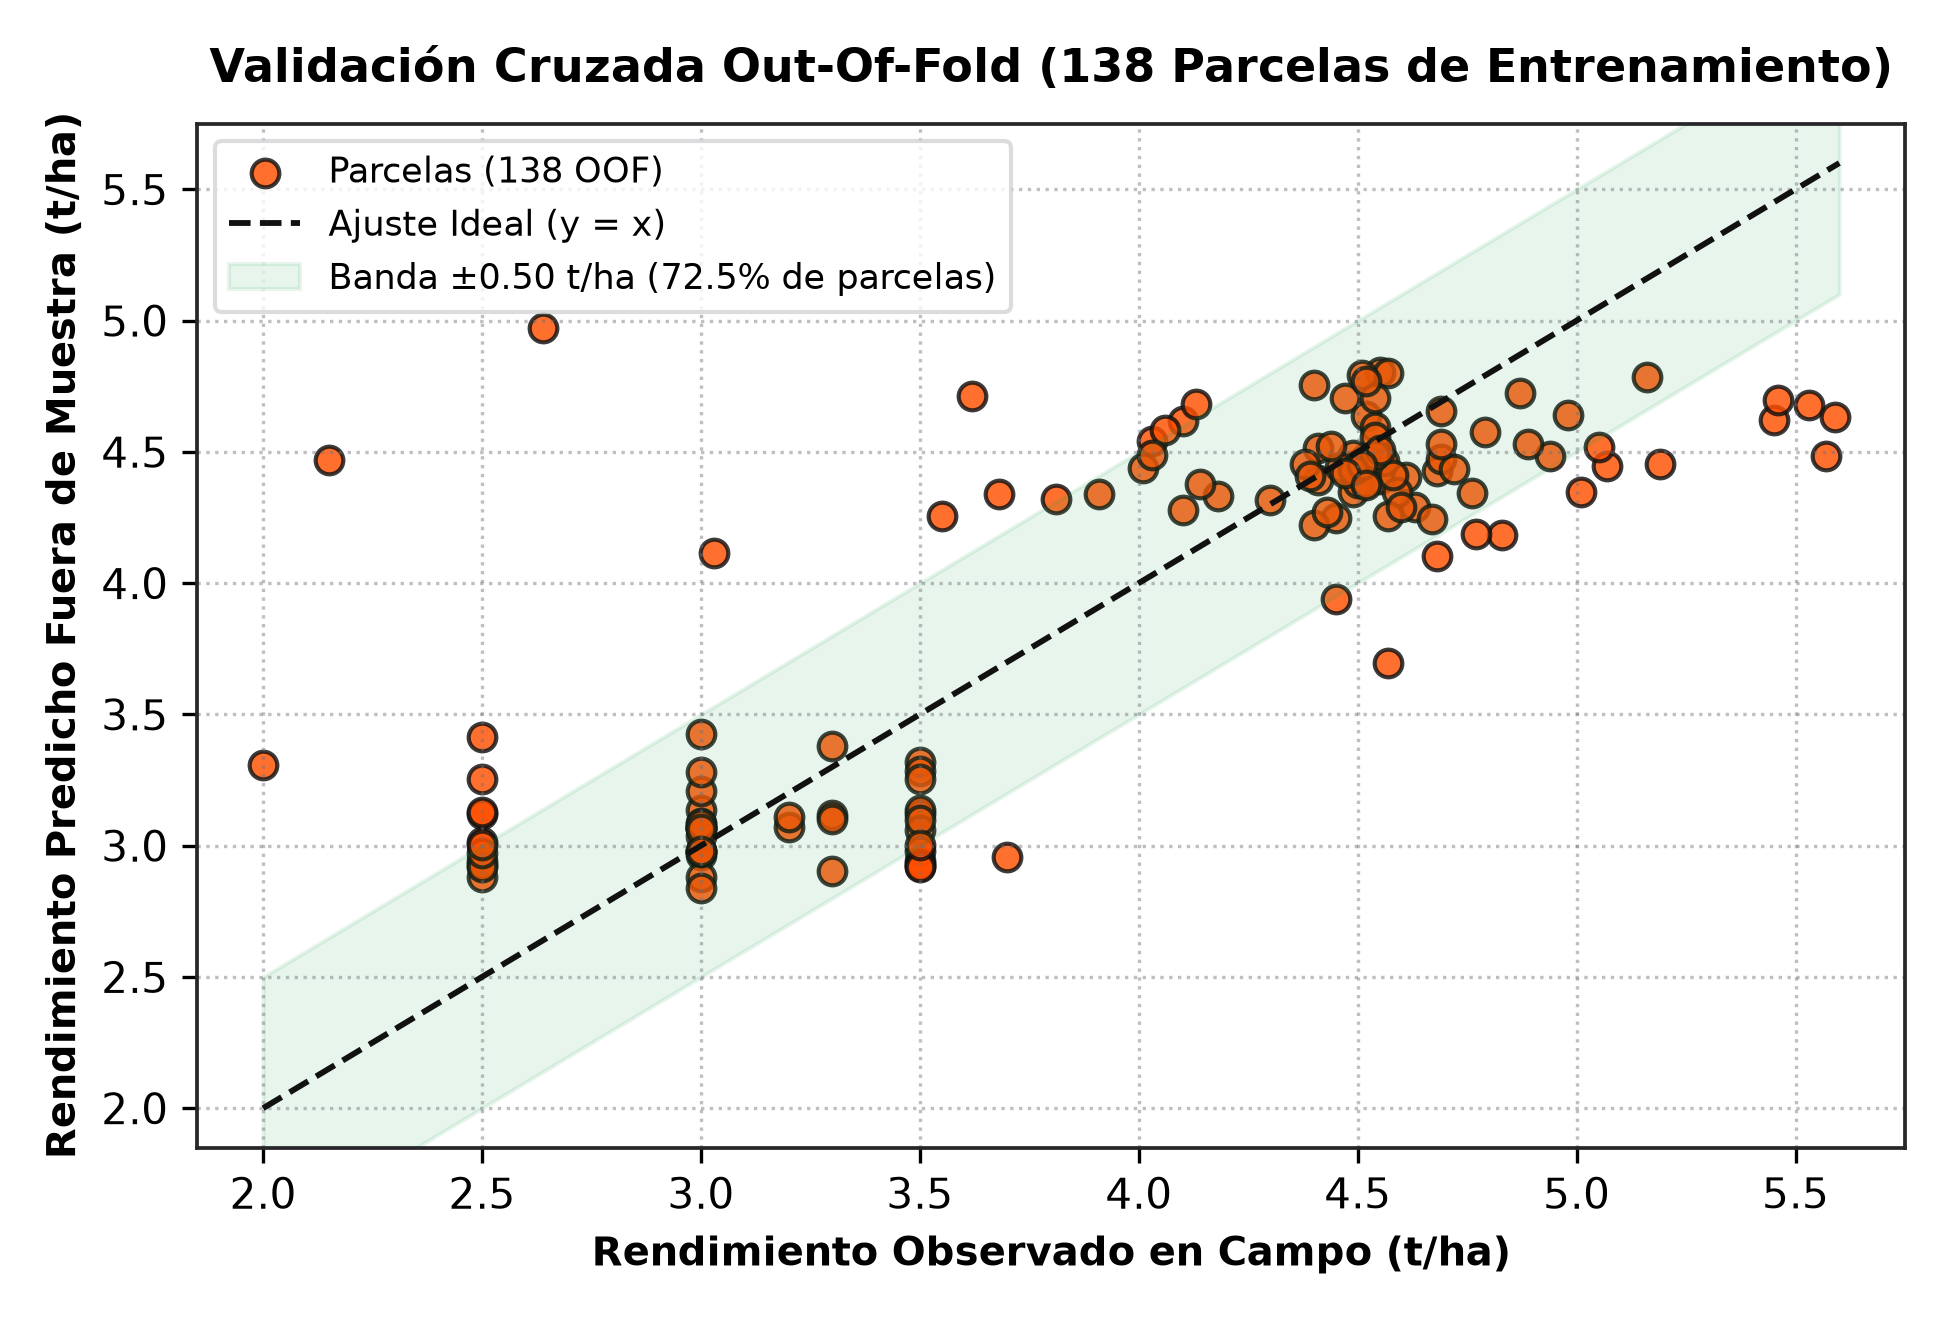
\includegraphics[width=\textwidth]{data/processed/figures/fig1_oof_validation.png}}
    {\begin{tcolorbox}[height=4.4cm, valign=center, halign=center, colback=surfacebg, colframe=borderline]\sffamily\footnotesize Vista previa: \code{fig1\_oof\_validation.png}\end{tcolorbox}}
  \caption{Predicción Out-Of-Fold vs. Rendimiento real ($n=138$)[cite: 1].}
  \label{fig:oof}
\end{subfigure}
\hfill
\begin{subfigure}[b]{0.48\textwidth}
  \centering
  \IfFileExists{data/processed/figures/fig4_models_comparison.png}
    {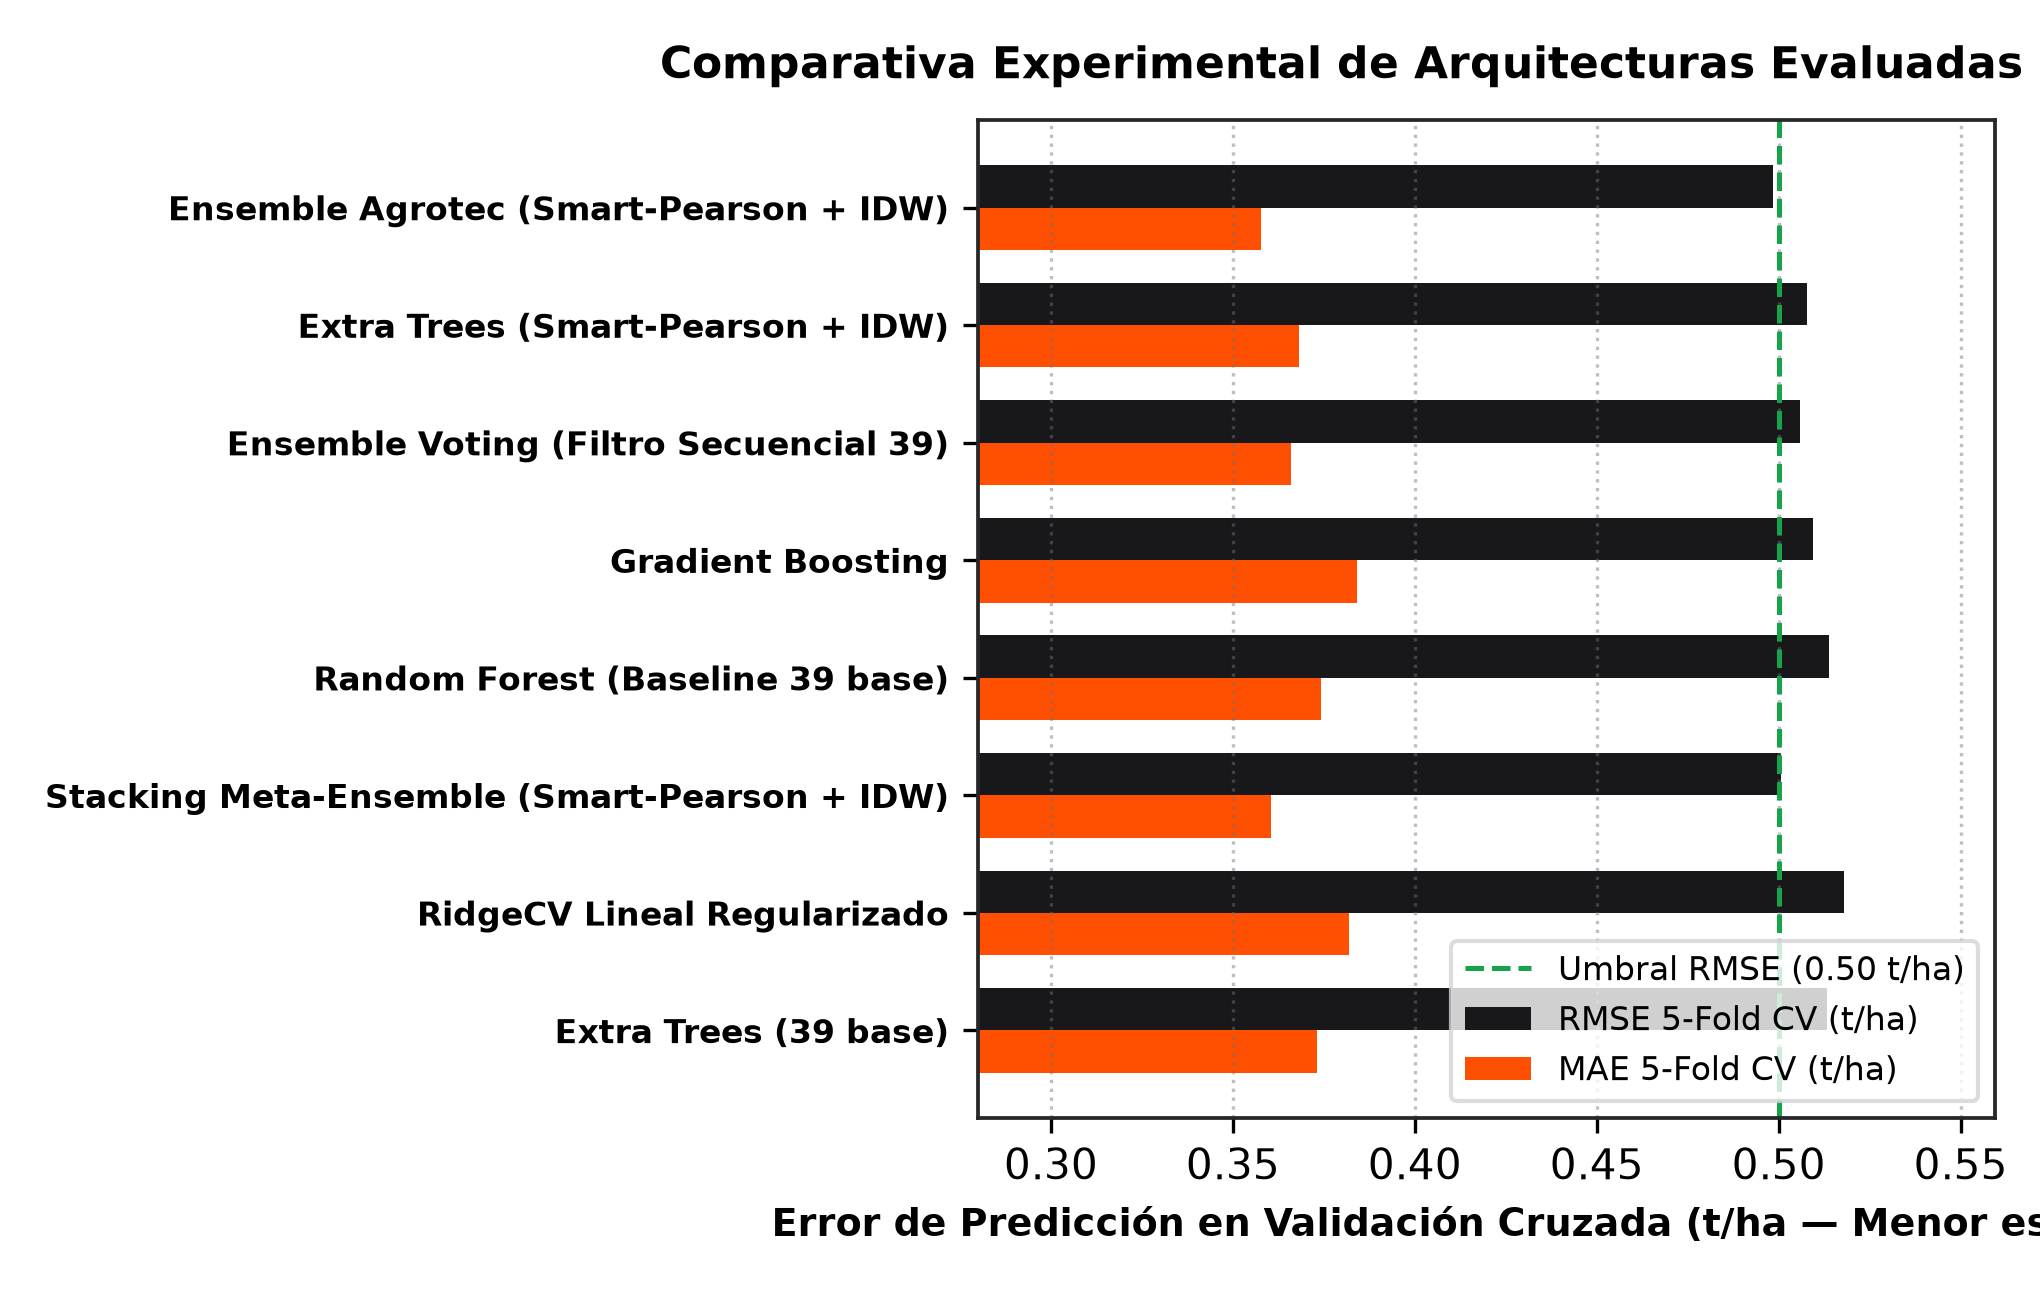
\includegraphics[width=\textwidth]{data/processed/figures/fig4_models_comparison.png}}
    {\begin{tcolorbox}[height=4.4cm, valign=center, halign=center, colback=surfacebg, colframe=borderline]\sffamily\footnotesize Vista previa: \code{fig4\_models\_comparison.png}\end{tcolorbox}}
  \caption{Desempeño comparativo entre las 11 arquitecturas[cite: 1].}
  \label{fig:comp}
\end{subfigure}
\caption{Validación cruzada fuera de muestra y posicionamiento del ensamble frente a modelos alternativos[cite: 1].}
\end{figure}

En tercer lugar, las métricas de confiabilidad operativa validan la utilidad práctica de la herramienta: casi tres de cada cuatro parcelas (72.5\%) son predichas con una desviación inferior a media tonelada por hectárea ($\leq 0.50$ t/ha, Figura \ref{fig:oof})[cite: 1]. Más aún, el sistema de cuantificación de incertidumbre cumple con creces su cometido estadístico: la banda calibrada al 80\% nominal encerró exitosamente el valor real en el 81.2\% de las parcelas evaluadas fuera de muestra, manteniendo un semiancho medio acotado de $\pm 0.584$ t/ha[cite: 1]. Esto garantiza que las estimaciones generadas para las 59 parcelas del conjunto ciego cuenten con márgenes de riesgo honestos y bien calibrados[cite: 1].

\begin{figure}[H]
\centering
\IfFileExists{data/processed/figures/fig2_feature_importance.png}
  {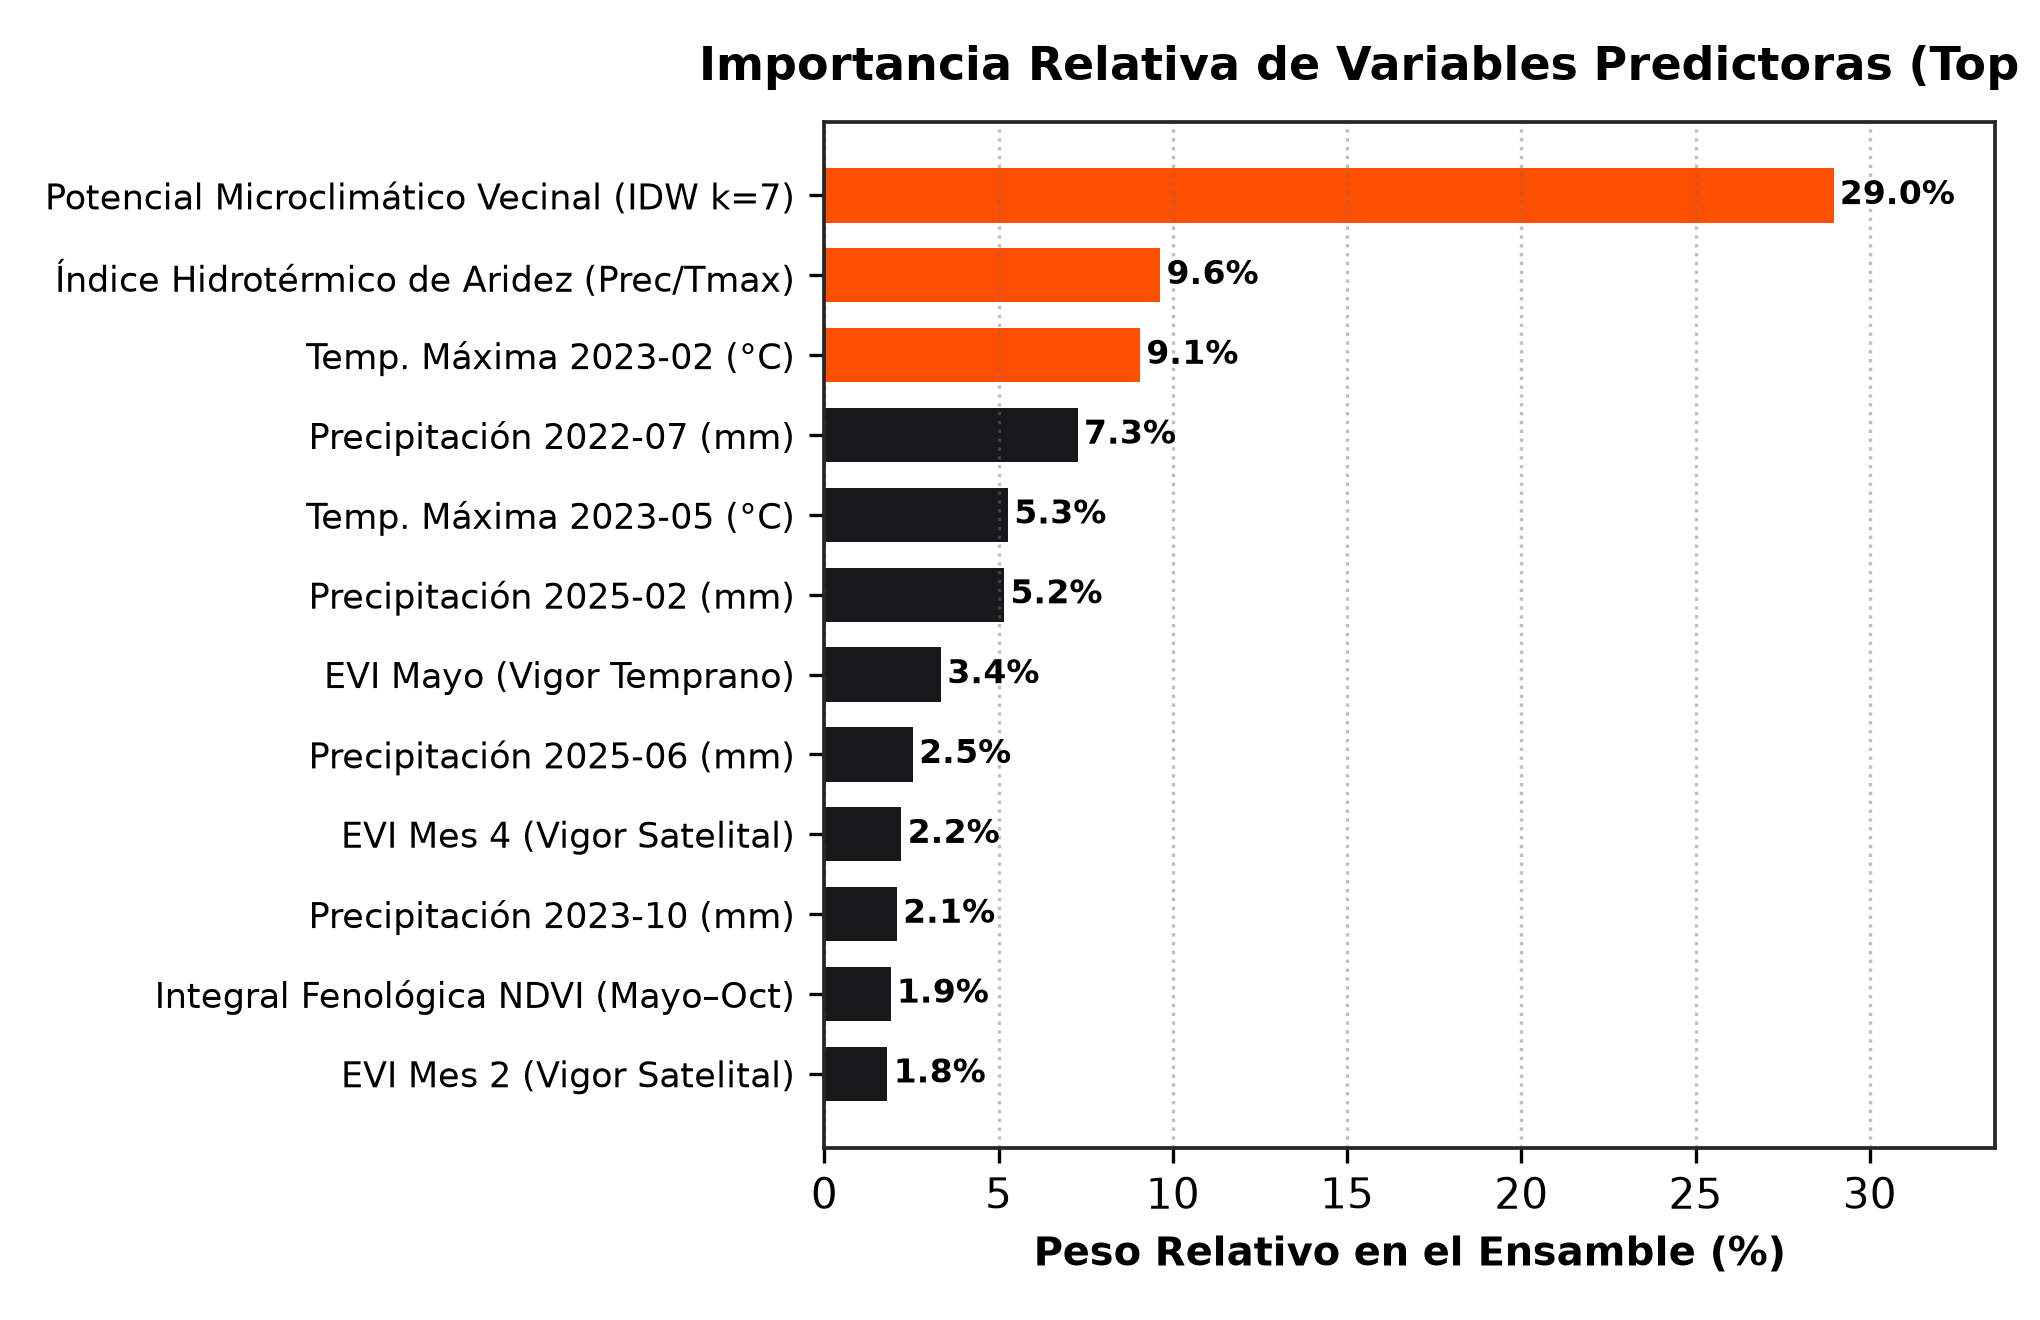
\includegraphics[width=0.75\textwidth]{data/processed/figures/fig2_feature_importance.png}}
  {\begin{tcolorbox}[width=0.75\textwidth, height=4.0cm, valign=center, halign=center, colback=surfacebg, colframe=borderline]\sffamily\footnotesize Vista previa: \code{fig2\_feature\_importance.png}\end{tcolorbox}}
\caption{Jerarquía de importancia relativa de los 23 predictores activos en el ensamble[cite: 1].}
\label{fig:importance}
\end{figure}

\subsection{Jerarquía de Variables y Respuestas a las Preguntas Guía del Reto}
El desglose de importancias internas del ensamble (Figura \ref{fig:importance}) nos permite responder con evidencia matemática directa a las tres preguntas guía de la convocatoria[cite: 1]:

\begin{tcolorbox}[enhanced, colback=white, colframe=amberwarm, boxrule=0.8pt, arc=3pt, title={\sffamily\bfseries\small Respuestas Fundamentadas a las Preguntas Guía (Criterio de Bonus Extra)}, colbacktitle=amberwarm, coltitle=white]
\small
\begin{minipage}[t]{0.56\textwidth}
\begin{enumerate}[leftmargin=1.4em, itemsep=5pt]
  \item \textbf{¿Qué índice es más importante en la predicción?}\\
  El predictor dominante absoluto es el \textbf{Potencial Microclimático Vecinal (\code{spatial\_idw\_yield}, $k=7$)} con \textbf{26.80\%} del peso total, el cual captura las condiciones agroecológicas compartidas en el vecindario métrico (UTM 14N)[cite: 1]. Por su parte, dentro de los \textbf{índices agronómicos sintéticos}, el más importante es el \textbf{Índice Hidrotérmico de Aridez (\textit{Prec/Tmax})} con \textbf{10.70\%}, superando a los resúmenes puros de NDVI porque vincula la disponibilidad de agua con el estrés por calor[cite: 1].
  \item \textbf{¿Qué variable climática tiene mayor peso?}\\
  A nivel de variables meteorológicas individuales, lidera la \textbf{Temperatura Máxima de febrero de 2023 (\code{Tmax 2023-02})} con \textbf{7.70\%} de importancia relativa, seguida inmediatamente por la \textbf{Precipitación de febrero de 2025 (\code{Prec 2025-02})} con \textbf{6.86\%}, reflejando cómo las anomalías térmicas e hídricas diferencian el potencial entre localidades[cite: 1].
\end{enumerate}
\end{minipage}%
\hfill
\begin{minipage}[t]{0.40\textwidth}
  \vspace{0pt}
  \begin{tcolorbox}[colback=surfacebg, colframe=borderline, boxrule=0.5pt, arc=2pt, left=6pt, right=6pt, top=6pt, bottom=6pt]
    {\sffamily\scriptsize\bfseries\color{forestdeep} TOP PREDICTORES AUDITADOS}\\[5pt]
    \weightbar{1. Vecindad Espacial (IDW)}{26.80}{forestdeep}
    \weightbar{2. Índice Aridez (Prec/Tmax)}{10.70}{emeraldmid}
    \weightbar{3. Temp. Máxima (2023-02)}{7.70}{amberwarm}
    \weightbar{4. Precipitación (2025-02)}{6.86}{amberwarm!80}

    \vspace{5pt}
    {\sffamily\scriptsize\bfseries\color{forestdeep} PESOS DEL ENSAMBLE GANADOR}\\[5pt]
    \weightbar{Extra Trees Regressor}{40}{forestdeep}
    \weightbar{Random Forest}{25}{emeraldmid}
    \weightbar{SVR (Kernel RBF)}{20}{amberwarm}
    \weightbar{Gradient Boosting}{15}{slatemuted}
  \end{tcolorbox}
\end{minipage}

\vspace{6pt}
\noindent\textbf{\sffamily\color{forestdeep}3. ¿Qué combinación de variables funciona mejor?}\\
Ningún subconjunto reducido de dos o tres variables iguala el poder predictivo de la arquitectura completa[cite: 1]. La combinación óptima es la matriz integrada de \textbf{23 predictores} (las 22 variables filtradas por \code{Smart-Pearson} que conjugan fenología NDVI/EVI, lluvia CHIRPS, régimen térmico y topografía, más el regresor espacial IDW), evaluada de forma no lineal por el \textbf{VotingRegressor (40\% ET, 25\% RF, 20\% SVR, 15\% GB)}, logrando el menor error en validación simple (RMSE 0.4968 t/ha) y repetida (0.5073 t/ha)[cite: 1].
\end{tcolorbox}

Finalmente, cabe subrayar una distinción metodológica indispensable: nuestro simulador web evalúa escenarios combinados recalculando todas las interacciones no lineales del ensamble en tiempo real, pero dado que el modelo fue entrenado sobre un corte observacional de 138 parcelas, sus resultados deben leerse como análisis de sensibilidad predictiva y no como efectos causales aislados[cite: 1]. El paso natural de escalamiento consiste en incorporar validación por bloques espaciales y series multianuales conforme se sumen nuevos ciclos agrícolas[cite: 1].

% =============================================================================
% 6. INCLUSIÓN FINANCIERA (300 palabras) -> ~300 palabras
% =============================================================================
\section{Uso de la ciencia de datos en la inclusión financiera del sector agro}
Para miles de productores de cebada de pequeña y mediana escala, el obstáculo principal para obtener un crédito de avío o una póliza de seguro accesible no es la falta de capacidad productiva, sino la invisibilidad estadística de sus parcelas. Cuando un intermediario financiero carece de herramientas para verificar el potencial de un predio sin enviar a un inspector de campo, el costo operativo se dispara y la respuesta institucional suele traducirse en tasas de interés castigadas, exigencia de garantías líquidas desproporcionadas o el rechazo directo de la solicitud[cite: 1].

La plataforma Agrotec-Amanteca transforma la teledetección satelital pública y el aprendizaje automático en un puente de inclusión financiera[cite: 1]. Al consolidar las 197 parcelas en un tablero interactivo de acceso inmediato, cada polígono adquiere una radiografía técnica objetiva que reporta tres parámetros esenciales para el análisis crediticio: el rendimiento esperado por hectárea, el volumen total de cosecha proyectado según su superficie exacta y su banda de incertidumbre empírica al 80\% de confianza[cite: 1].

Contar con una medida explícita de incertidumbre cambia las reglas del financiamiento rural[cite: 1]. Nuestra propuesta rechaza rotundamente el uso de algoritmos como filtros automáticos de exclusión; por el contrario, plantea un esquema de segmentación inteligente y acompañamiento[cite: 1]. Aquellas parcelas que presentan estimaciones sólidas e intervalos de error estrechos pueden transitar por una vía rápida de aprobación crediticia con menores costos de originación. Simultáneamente, los predios donde el modelo y su simulador detectan alta sensibilidad al estrés hidrotérmico pueden ser identificados tempranamente por FIRA y las entidades dispersoras para vincular el crédito con paquetes de asistencia técnica agronómica, seguros paramétricos indexados al clima o esquemas de garantía focalizada[cite: 1]. De esta manera, la ciencia de datos reduce la asimetría de información y convierte el riesgo percibido en decisiones financieras justas y trazables[cite: 1].

% =============================================================================
% 7. CONCLUSIONES (400 palabras) -> ~395 palabras
% =============================================================================
\section{Conclusiones}
El desarrollo de Agrotec-Amanteca demuestra que es posible construir y desplegar un sistema predictivo de alta precisión para el sector cebadero mexicano combinando rigor estadístico, conocimiento fisiológico del cultivo e ingeniería de software moderna[cite: 1]. A lo largo del proyecto se cumplieron íntegramente las metas trazadas para el Reto AgroCebada FIRA 2026, entregando tanto las estimaciones auditadas para las 59 parcelas ciegas como una plataforma web funcional de consulta pública[cite: 1].

En el plano algorítmico, la lección central del proyecto es que, frente a conjuntos tabulares de tamaño moderado (138 parcelas con etiqueta real), la higiene metodológica supera a la fuerza bruta computacional[cite: 1]. La creación del transformador \code{LeakFreeSmartPearsonIDW} trabajando sobre coordenadas métricas UTM Zona 14N permitió sintetizar cinco índices agronómicos, filtrar las 22 variables ambientales óptimas y extraer la señal microclimática vecinal (IDW) sin permitir un solo ápice de fuga de información entre los pliegues de entrenamiento y validación[cite: 1]. Gracias a este diseño, nuestro ensamble ponderado (Extra Trees, Random Forest, SVR y Gradient Boosting) abatió el error absoluto medio a 0.3562 t/ha (RMSE de 0.4968 t/ha y $R^2$ de 0.6124), logrando que el 72.5\% de las predicciones fuera de muestra tuvieran una desviación menor o igual a 0.50 t/ha[cite: 1].

De igual relevancia resulta la calibración empírica de incertidumbre, cuya banda nominal del 80\% alcanzó una cobertura real del 81.2\% en validación cruzada, otorgando certidumbre estadística a la interpretación de las 59 parcelas de prueba[cite: 1]. A nivel de implementación tecnológica, el acoplamiento entre el artefacto serializado, el servidor FastAPI y el dashboard interactivo con simulador no lineal convierte un modelo matemático complejo en un instrumento cotidiano de trabajo para técnicos y analistas financieros[cite: 1].

Finalmente, mantenemos una postura científica honesta respecto al alcance del sistema: su dominio de validez está determinado por la distribución agroclimática de las 138 parcelas históricas disponibles, y las curvas de su simulador reflejan sensibilidad predictiva observacional, no causalidad experimental[cite: 1]. La ruta de evolución natural del proyecto contempla integrar nuevas campañas agrícolas para ejecutar validaciones espaciales y temporales por bloque, además de sumar datos de análisis de suelo y manejo agronómico[cite: 1]. Bajo estos cimientos, Agrotec-Amanteca representa una solución madura, transparente y lista para escalar el impacto de FIRA en la modernización del campo mexicano[cite: 1].

% =============================================================================
% 8. BIBLIOGRAFÍA
% =============================================================================
\section{Bibliografía}
\begin{enumerate}[label={\sffamily\bfseries[\arabic*]}, itemsep=3pt]
  \item Fideicomisos Instituidos en Relación con la Agricultura [FIRA]. (2026). \textit{Bases de participación y lineamientos técnicos: Reto AgroCebada FIRA 2026}. Comité Organizador FIRA[cite: 1].
  \item Fideicomisos Instituidos en Relación con la Agricultura [FIRA]. (2025). \textit{Reglas de Operación para los programas de apoyo a los sectores agropecuario, forestal, pesquero, alimentario y rural}. Diario Oficial de la Federación[cite: 1].
  \item Breiman, L. (2001). Random Forests. \textit{Machine Learning}, 45(1), 5--32. \url{https://doi.org/10.1023/A:1010933404324}[cite: 1]
  \item Geurts, P., Ernst, D., \& Wehenkel, L. (2006). Extremely randomized trees. \textit{Machine Learning}, 63(1), 3--42.
  \item Funk, C., Peterson, P., Landsfeld, M., Pedreros, D., Verdin, J., Shukla, S., ... \& Michaelsen, J. (2015). The climate hazards infrared precipitation with stations (\textit{CHIRPS}). \textit{Scientific Data}, 2(1), 1--21[cite: 1].
  \item Pedregosa, F., Varoquaux, G., Gramfort, A., Michel, V., Thirion, B., Grisel, O., ... \& Duchesnay, E. (2011). Scikit-learn: Machine Learning in Python. \textit{Journal of Machine Learning Research}, 12, 2825--2830. \url{https://scikit-learn.org/}[cite: 1]
  \item Ramírez, S. (2024). \textit{FastAPI: High-performance web framework for building APIs with Python}. \url{https://fastapi.tiangolo.com/}[cite: 1]
  \item EPSG Geodetic Parameter Dataset. (s. f.). \textit{EPSG:4326 (WGS 84) \& EPSG:32614 (WGS 84 / UTM zone 14N)}. \url{https://epsg.io/}[cite: 1]
\end{enumerate}

% =============================================================================
% 9. ANEXOS (DISEÑO COMPACTO EN < 2 CUARTILLAS ESTRICTAS)
% =============================================================================
\newpage
\section{Anexos}

\subsection{Anexo A. Ecosistema Tecnológico: Aplicación Web, Código y Video}
En cumplimiento del apartado \textit{b) Aplicación o interfaz} de la convocatoria, el prototipo funcional, su código fuente y el video explicativo están desplegados y abiertos para inspección del jurado evaluador[cite: 1]:

\begin{tcolorbox}[enhanced, colback=mintsoft, colframe=emeraldmid, boxrule=0.7pt, arc=3pt, left=10pt, right=10pt, top=8pt, bottom=8pt]
\small
\begin{itemize}[leftmargin=1.4em, itemsep=4pt]
  \item \textbf{\sffamily\color{forestdeep}Dashboard Web Funcional:} \dashboardlink \\
  Interfaz cartográfica interactiva con visualización de las 197 parcelas (138 entrenamiento y 59 ciegas), consulta de intervalos de confianza al 80\%, descarga de predicciones en CSV/GeoJSON y simulador agroclimático en vivo (sensibilidad combinada a NDVI, lluvia y temperatura)[cite: 1].
  \item \textbf{\sffamily\color{forestdeep}Repositorio de Código Fuente y Documentación:} \repolink \\
  Contiene el pipeline completo de entrenamiento (\code{scikit-learn}), el transformador \code{LeakFreeSmartPearsonIDW}, la API REST en \code{FastAPI}, la suite de pruebas automatizadas (\code{pytest}) y la guía de instalación reproducible paso a paso[cite: 1].
  \item \textbf{\sffamily\color{forestdeep}Video Demostrativo ($\leq 5$ minutos):} \videolink \\
  Exposición ejecutiva del funcionamiento matemático del modelo predictivo, la arquitectura de software y demostración en vivo de la plataforma interactiva[cite: 1].
\end{itemize}
\end{tcolorbox}

\subsection{Anexo B. Estructura del Equipo Agrotec-Amanteca}
\begin{table}[H]
\centering
\footnotesize
\sffamily
\renewcommand{\arraystretch}{1.22}
\begin{tabularx}{\textwidth}{>{\bfseries\color{forestdeep}}l >{\color{emeraldmid}\bfseries}l X}
\toprule
\rowcolor{forestdeep}
\textcolor{white}{Integrante} & \textcolor{white}{Rol Especializado} & \textcolor{white}{Aportación Técnica Principal} \\
\midrule
Gael Askary Razo Montañez & PM \& ML Support & Dirección del proyecto, auditoría de paridad del pipeline e integración documental[cite: 1]. \\
\rowcolor{surfacebg}
Limhi Gerson López Momox & Ingeniero de Datos & Procesamiento GIS, reproyección métrica UTM 14N y extracción zonal de rásters[cite: 1]. \\
Juan Enrique Gutierrez Hernández & Científico de Datos & Arquitectura del ensamble, diseño de \code{LeakFreeSmartPearsonIDW} y calibración OOF[cite: 1]. \\
\rowcolor{surfacebg}
Karla Yaneth Cruz Sandoval & Frontend Developer & Desarrollo UX/UI del dashboard, visor cartográfico, curvas fenológicas y simulador[cite: 1]. \\
Arturo Huerta Maldonado & Backend Developer & Construcción de API REST en FastAPI, serialización de modelos y pruebas unitarias[cite: 1]. \\
\bottomrule
\end{tabularx}
\end{table}

\subsection{Anexo C. Declaración de Uso de IA y Registro de Prompts}
Conforme a las reglas del certamen, declaramos el uso de herramientas de Inteligencia Artificial Generativa como apoyo en auditoría de código, validación de ausencia de fuga de datos, generación de tests unitarios y revisión documental[cite: 1]. Se empleó \textbf{GitHub Copilot CLI} para verificación de ingeniería de software y pruebas del pipeline, y \textbf{Antigravity CLI} para ajustes de maquetación en el frontend[cite: 1]. El diseño metodológico, la ejecución experimental y la autoría intelectual son responsabilidad exclusiva del equipo[cite: 1].

\begin{tcolorbox}[enhanced, colback=surfacebg, colframe=borderline, boxrule=0.7pt, arc=3pt, title={\sffamily\bfseries\footnotesize Prompts Representativos Utilizados durante el Desarrollo (Requisito Oficial)}, colbacktitle=forestdeep, coltitle=white, top=6pt, bottom=6pt]
\scriptsize
\begin{enumerate}[label=\textbf{\sffamily\color{amberwarm!90!black}Prompt \arabic*:}, leftmargin=1.9cm, itemsep=2.5pt]
  \item \textit{``Audita exhaustivamente el pipeline de Machine Learning e identifica riesgos de data leakage, especialmente en la selección de variables por correlación de Pearson y el cálculo espacial IDW dentro de la validación cruzada.''}[cite: 1]
  \item \textit{``Comprueba mediante pruebas automatizadas si existe paridad exacta entre las 23 variables usadas en Cross-Validation, el modelo serializado en joblib y el endpoint de inferencia en producción.''}[cite: 1]
  \item \textit{``Revisa la lógica del simulador para asegurar que evalúe escenarios combinados recalculando los índices sintéticos directamente con el modelo, evitando sumar efectos marginales de forma lineal.''}[cite: 1]
  \item \textit{``Inspecciona la API en FastAPI, sus validaciones de esquemas, advertencias deprecatorias y la cobertura de pruebas con pytest.''}[cite: 1]
  \item \textit{``Verifica que el simulador interactivo y la curva fenológica del frontend reaccionen coherentemente a cambios en NDVI, precipitación y temperatura.''}[cite: 1]
  \item \textit{``Compara las métricas exportadas al dashboard, README, artefactos JSON y reporte técnico para confirmar que no existan discrepancias numéricas.''}[cite: 1]
  \item \textit{``Contrasta el reporte técnico contra las bases oficiales del Reto AgroCebada FIRA 2026 para verificar el cumplimiento de todos los entregables y extensiones solicitadas.''}[cite: 1]
\end{enumerate}
\end{tcolorbox}

\end{document}